%==========================================================================
% DESIGN COMPONENTS
%==========================================================================
\section{Design Components}
\label{sec:design}
%
%==========================================================================
% OVERIVEW
%==========================================================================
%
\subsection{System Overview}
%

%


%==========================================================================
% PROTECTION DOMAINS
%==========================================================================
%
\subsection{Protection Domains}
%
Our \textit{fault model} for memory protection is the corruption of state belonging to other user modules caused due to illegal write operations made by any one of the modules.
%
We create and enforce \emph{Protection Domains} within data memory address space of sensor node.
%
Protection domain refers to a fragmented but logically distinct portion of overall data memory address space (Figure ~\ref{fig:prot_domains}).
%
Every module stores its state in separate protection domain.
%
No assumptions are made about layout of state belonging to individual modules within their domain.
%
Modules are restricted from writing to memory outside their domain through run-time checks.
%
There is one single trusted domain that can access all memory.
%

Protection model based on domains does not address all possible memory corruption faults in the system.
%
Modules can still corrupt their own state as it resides completely within a protection domain. 
%
This form of corruption, though undesirable, is less serious than corruption across domains.
%
If we have an operating system, we can load the kernel image in the single trusted domain.
%
A stable kernel can always ensure a clean re-start of user modules when corruption is detected.
%
\begin{figure}[htbp]
   \centering
   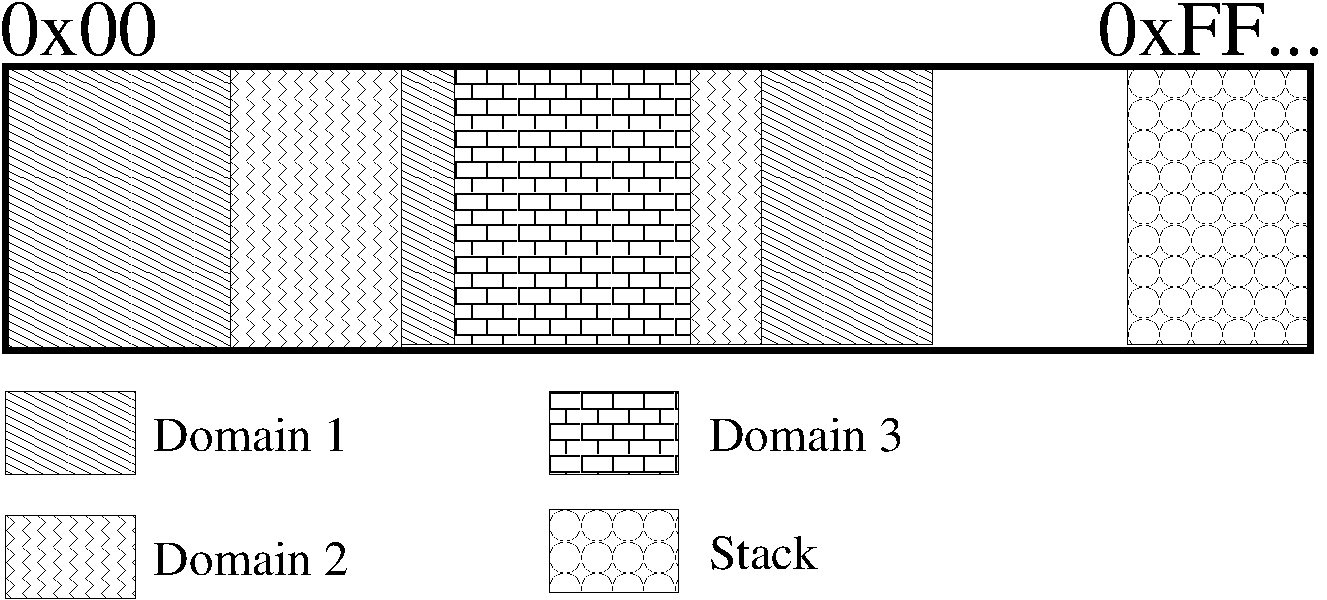
\includegraphics[height = 1in, keepaspectratio=true]{figures/domains.pdf} 
   \caption{Protection Domains}
   \label{fig:prot_domains}
\end{figure}
%
%========================================================================================================================================
% MEMORY MAP DATA STRUCTURE
%========================================================================================================================================
\subsection{Memory Map}
%
%
Creating and enforcing protection domains is a challenging task on resource constrained embedded platforms.
%
Limited memory prohibits static contiguous partitioning of address space into multiple domains.
%
Instead we partition the address space of the microcontroller into blocks of equal sizes.
%
\textit{Block} is a small contiguous region of memory.
%
Memory is allocated to domains as \textit{segments}; a set of contiguous blocks.
%
Allocation of segments to domains could be static (at compile time) or dynamic (through \texttt{malloc}).
%
A domain could be allocated multiple segments that are scattered randomly across entire address space.
%
\textit{Memory map contains access permissions for every block of address space.}
%
Memory map specifies two pieces of information.
% 
First, it contains ownership information (domain identity) for every block of memory.
%
Second, it encodes information about memory layout such as start of a logical segment of allocation to programs.
%
An example of actual encoded information and their meaning is specified in Table~\ref{tab:mmap_table}.
%
\begin{table}[htdp]
\centering
\small{
\begin{tabular}{|c|l|}
	\hline
	Code & Meaning\\
	\hline
	1111 & Free or Start of Trusted Segment\\
	1110 & Later portion of Trusted Segment\\
	xxx1 & Start of Domain (0 - 6) Segment \\
	xxx0 & Later portion of Domain (0 - 6) Segment\\
	\hline
\end{tabular}}
\caption{Encoded information in memory map table for multi-domain protection}
\label{tab:mmap_table}
\end{table}

%
Base pointer of memory map is stored in a special register called \texttt{MMP\_BASE\_PTR}.
%
Mapping from the address to the memory map is shown in Figure~\ref{fig:addr_memmap_translate}.
%
Assuming block size of 8 bytes, last three bits of address are offset into a given block.
%
Remaining bits represent block number in data memory.
%
Permissions are packed into a byte.
%
If encoded information is stored in four bits (for multi-domain protection), then each byte would contain information of two contiguous memory blocks.
%
Therefore, last bit of block number represents byte offset of permission.
%
Remaining bits index into memory map table.
%
This particular design of memory map table was chosen to minimize memory footprint.
%
%
%
\begin{figure}[htbp]
   \centering
   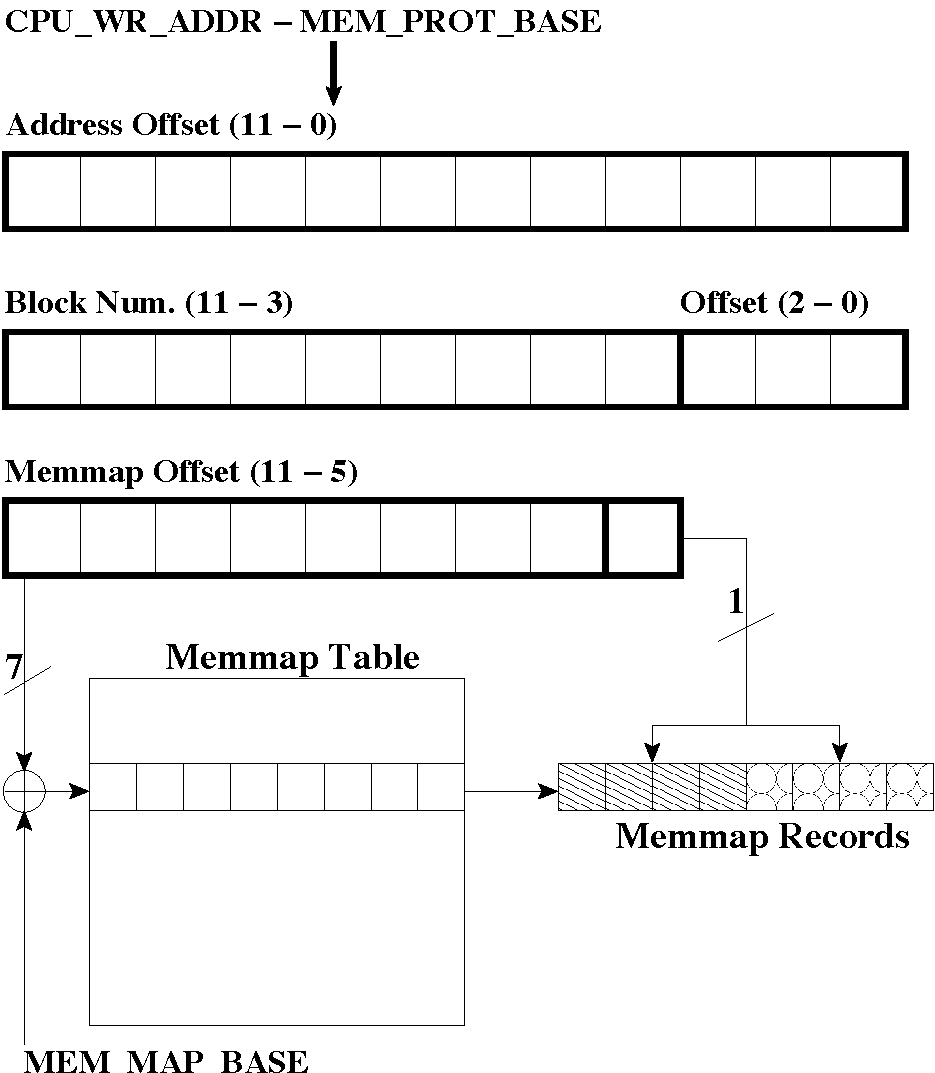
\includegraphics[height=1.75in, keepaspectratio=true]{figures/memaddrtrans.pdf} 
   \caption{Address to memory map translation}
   \label{fig:addr_memmap_translate}
\end{figure}
%
% If we optimize the memory map table to not include certain portions of the address space, then what will happen if we accidentally pass an unmapped address ?
%
%
%
%\begin{table*}
%   \centering
%   \small{
%   \begin{tabular}{|l|l|}
%   \hline
%   Prototype & Description \\
%   \hline
%   int8\_t memmap\_set(uint8\_t blkID, uint8\_t nBlks, uint8\_t domID) & Set owner of segment [BlkID, BlkID + nBlks) to domID \\
%   \hline
%   uint8\_t memmap\_get(uint8\_t blkID) & Get owner and layout of block number BlkID \\
%   \hline
%   \end{tabular}
%   }
%   \centering
%   \caption{Memory Map API}
%   \label{tab:memmap_api}
%\end{table*}
%
%
%========================================================================================================================================
% MEMORY MAP CHECKER
%========================================================================================================================================
\subsection{Memory Map Checker}
%
A run-time checker is required to validate memory accesses made by software components.
%
Memory accesses need to be validated against a protection model.
%
Our memory map checker enforces the protection model that we described earlier; programs can write only into their domain.
%
%A single trusted domain in the system is allowed to access all memory.
%
The run-time is a functional unit that in invoked when the store instruction is executed by the processor.
%
The checker then performs three operations when invoked.
%
First, the checker stalls the processor execution and takes control of the address bus to memory.
%
Second, it retrieves the byte containing ownership information from memory map table for the current store address.
%
The address translation shown in Figure~\ref{fig:addr_memmap_translate}.% is performed within a single clock cycle and a read is issued to the memory.
%
%The ownership byte is received in the next clock cycle.
%
Third, the checker compares the ownership information to the identity of the current executing domain.
%
It triggers an exception on failure, else it resumes the execution of the processor.
%
All these operations add a delay of one clock cycle to the store operation.
%
The address translation is performed in the same clock cycle as the store instruction begins execution.
%
The read of ownership byte from memory map takes one clock cycles.
%
Comparison of the ownership byte is performed within a clock cycle and the processor execution is resumed immediately upon success.
%
%========================================================================================================================================
% MEMORY MAP FOR PROTECTION
%========================================================================================================================================
\subsection{Memory Map Software Library}
\label{subsec:mmap_for_protection}
%
Memory map software library provides routines that enable various protection models in the microcontroller.
%
%Memory map data structure and address translation operations are encapsulated into an object that is accessible through an API described in Table~\ref{tab:memmap_api}. 	
%
%This API is located in the single trusted domain in the system and is not accessible to software modules present in other domains.
%
The software library ensures following conditions.
%
First, it ensures that the memory map accurately reflects current ownership and layout.
%
In any real system, memory is constantly allocated, de-allocated or transferred from one module to another.
%
Memory map should be immediately updated when any of these events occur.
%
The library provides \texttt{malloc}, \texttt{free} and \texttt{change\_own} calls that automatically update memory map data structure. 
%
Second, it only permits the  block owner to free or change its ownership.
%
This condition is necessary as one module may accidentally (due to programming errors) free up memory that is being used by other module in the system.
%
Also it prevents a module from accidentally hijacking memory that is owned by other modules.
%
To enforce this condition, the software needs to track the current active domain.
%
We describe implementation details of tracking current active application in Section~\ref{sec:cfmgr}.
%
Third, the software library sets up the memory map to be located in a protected region of memory.
%
This prevents accidental corruption of memory map data structure.
%








